
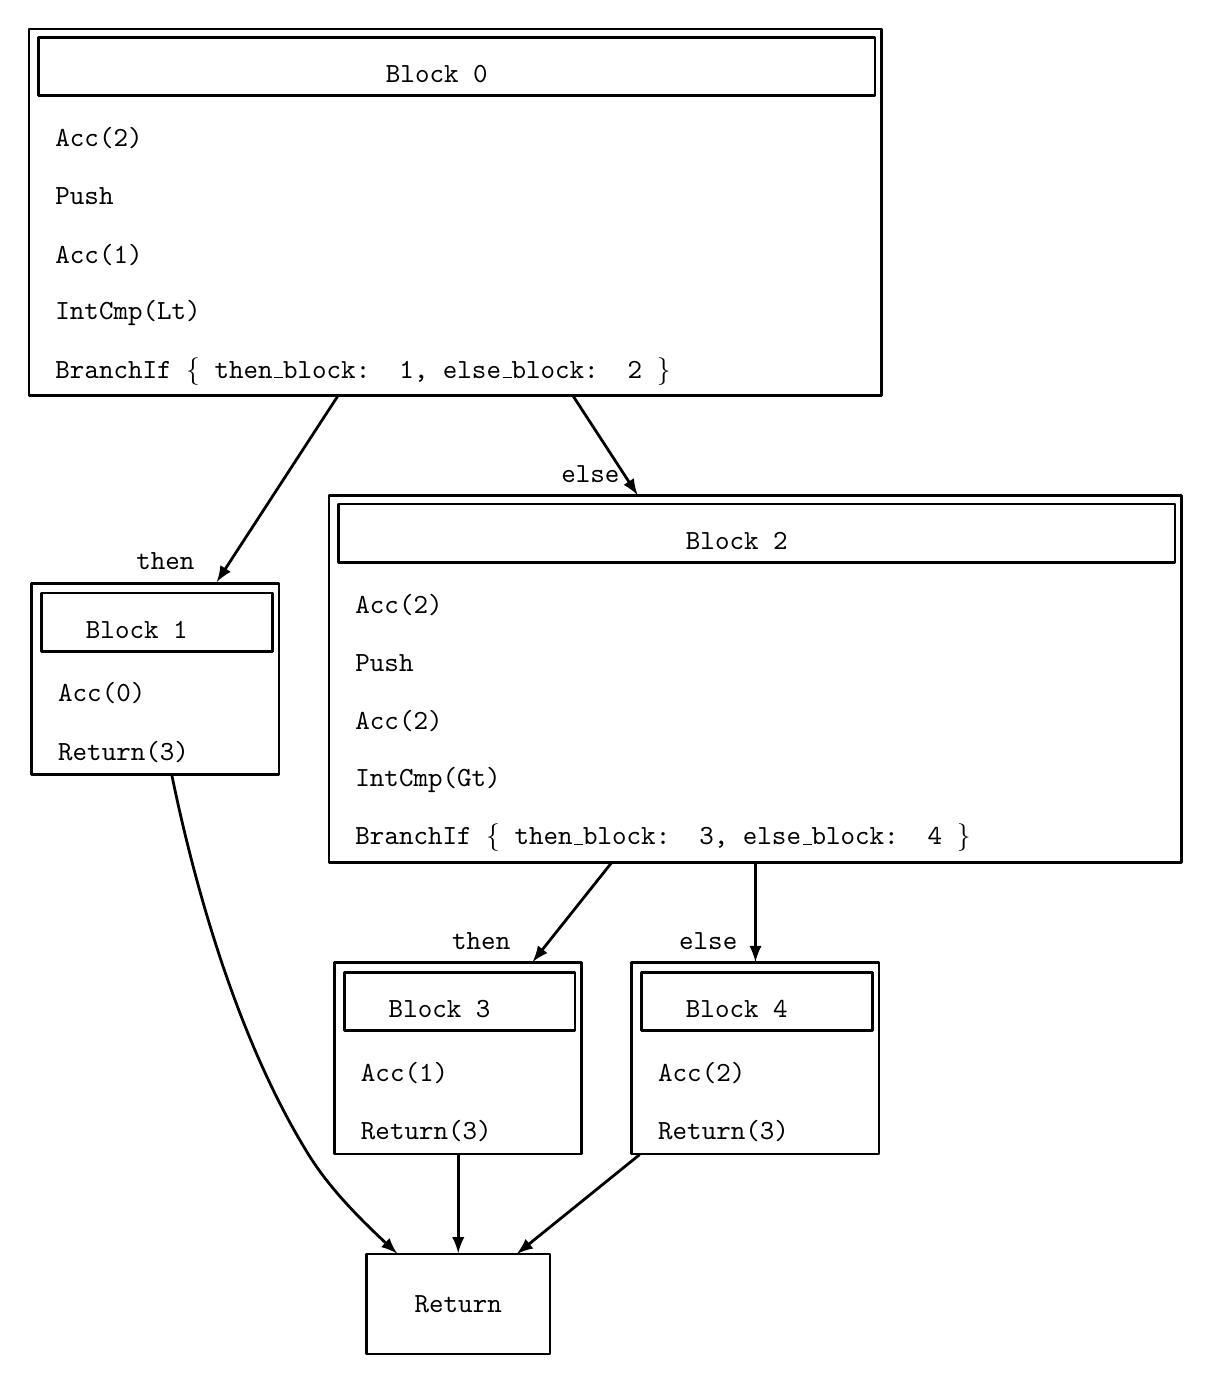
\begin{tikzpicture}[>=latex,line join=bevel,]
  \pgfsetlinewidth{1bp}
\ttfamily%
\pgfsetcolor{black}
  % Edge: n0 -> n1
  \draw [->] (111.13bp,344.87bp) .. controls (98.328bp,325.2bp) and (84.615bp,304.12bp)  .. (67.561bp,277.91bp);
  \definecolor{strokecol}{rgb}{0.0,0.0,0.0};
  \pgfsetstrokecolor{strokecol}
  \draw (49.061bp,285.41bp) node { then};
  % Edge: n0 -> n2
  \draw [->] (195.87bp,344.87bp) .. controls (201.65bp,335.99bp) and (207.61bp,326.82bp)  .. (219.07bp,309.22bp);
  \draw (202.07bp,316.72bp) node { else};
  % Edge: n1 -> return
  \draw [->] (51.405bp,208.35bp) .. controls (58.789bp,172.52bp) and (73.825bp,115.14bp)  .. (100.5bp,72.0bp) .. controls (107.02bp,61.458bp) and (116.07bp,51.486bp)  .. (132.53bp,36.158bp);
  % Edge: n2 -> n3
  \draw [->] (209.57bp,176.72bp) .. controls (202.07bp,167.29bp) and (194.52bp,157.81bp)  .. (181.28bp,141.16bp);
  \draw (162.78bp,148.66bp) node { then};
  % Edge: n2 -> n4
  \draw [->] (261.5bp,176.72bp) .. controls (261.5bp,168.06bp) and (261.5bp,159.36bp)  .. (261.5bp,141.16bp);
  \draw (244.5bp,148.66bp) node { else};
  % Edge: n3 -> return
  \draw [->] (154.5bp,71.809bp) .. controls (154.5bp,63.365bp) and (154.5bp,54.41bp)  .. (154.5bp,36.297bp);
  % Edge: n4 -> return
  \draw [->] (219.82bp,71.809bp) .. controls (207.64bp,61.961bp) and (194.6bp,51.416bp)  .. (175.6bp,36.059bp);
  % Node: n0
\begin{scope}
  \definecolor{strokecol}{rgb}{0.0,0.0,0.0};
  \pgfsetstrokecolor{strokecol}
  \draw (3.5bp,453.0bp) -- (3.5bp,474.0bp) -- (304.5bp,474.0bp) -- (304.5bp,453.0bp) -- cycle;
  \draw (124.5bp,460.8bp) node[right] {Block 0};
  \draw (5.5bp,437.8bp) node[right] {Acc(2)  };
  \draw (5.5bp,416.8bp) node[right] {Push  };
  \draw (5.5bp,395.8bp) node[right] {Acc(1)  };
  \draw (5.5bp,374.8bp) node[right] {IntCmp(Lt)  };
  \draw (5.5bp,353.8bp) node[right] {BranchIf \{ then\_block: 1, else\_block: 2 \}  };
  \draw (0.0bp,345.0bp) -- (0.0bp,477.0bp) -- (307.0bp,477.0bp) -- (307.0bp,345.0bp) -- cycle;
\end{scope}
  % Node: n1
\begin{scope}
  \definecolor{strokecol}{rgb}{0.0,0.0,0.0};
  \pgfsetstrokecolor{strokecol}
  \draw (4.5bp,253.0bp) -- (4.5bp,274.0bp) -- (87.5bp,274.0bp) -- (87.5bp,253.0bp) -- cycle;
  \draw (16.5bp,260.8bp) node[right] {Block 1};
  \draw (6.5bp,237.8bp) node[right] {Acc(0)  };
  \draw (6.5bp,216.8bp) node[right] {Return(3)  };
  \draw (1.0bp,208.5bp) -- (1.0bp,277.5bp) -- (90.0bp,277.5bp) -- (90.0bp,208.5bp) -- cycle;
\end{scope}
  % Node: n2
\begin{scope}
  \definecolor{strokecol}{rgb}{0.0,0.0,0.0};
  \pgfsetstrokecolor{strokecol}
  \draw (111.5bp,285.0bp) -- (111.5bp,306.0bp) -- (412.5bp,306.0bp) -- (412.5bp,285.0bp) -- cycle;
  \draw (232.5bp,292.8bp) node[right] {Block 2};
  \draw (113.5bp,269.8bp) node[right] {Acc(2)  };
  \draw (113.5bp,248.8bp) node[right] {Push  };
  \draw (113.5bp,227.8bp) node[right] {Acc(2)  };
  \draw (113.5bp,206.8bp) node[right] {IntCmp(Gt)  };
  \draw (113.5bp,185.8bp) node[right] {BranchIf \{ then\_block: 3, else\_block: 4 \}  };
  \draw (108.0bp,177.0bp) -- (108.0bp,309.0bp) -- (415.0bp,309.0bp) -- (415.0bp,177.0bp) -- cycle;
\end{scope}
  % Node: return
\begin{scope}
  \definecolor{strokecol}{rgb}{0.0,0.0,0.0};
  \pgfsetstrokecolor{strokecol}
  \draw (187.5bp,36.0bp) -- (121.5bp,36.0bp) -- (121.5bp,0.0bp) -- (187.5bp,0.0bp) -- cycle;
  \draw (154.5bp,18.0bp) node {Return};
\end{scope}
  % Node: n3
\begin{scope}
  \definecolor{strokecol}{rgb}{0.0,0.0,0.0};
  \pgfsetstrokecolor{strokecol}
  \draw (113.5bp,116.5bp) -- (113.5bp,137.5bp) -- (196.5bp,137.5bp) -- (196.5bp,116.5bp) -- cycle;
  \draw (125.5bp,124.3bp) node[right] {Block 3};
  \draw (115.5bp,101.3bp) node[right] {Acc(1)  };
  \draw (115.5bp,80.3bp) node[right] {Return(3)  };
  \draw (110.0bp,72.0bp) -- (110.0bp,141.0bp) -- (199.0bp,141.0bp) -- (199.0bp,72.0bp) -- cycle;
\end{scope}
  % Node: n4
\begin{scope}
  \definecolor{strokecol}{rgb}{0.0,0.0,0.0};
  \pgfsetstrokecolor{strokecol}
  \draw (220.5bp,116.5bp) -- (220.5bp,137.5bp) -- (303.5bp,137.5bp) -- (303.5bp,116.5bp) -- cycle;
  \draw (232.5bp,124.3bp) node[right] {Block 4};
  \draw (222.5bp,101.3bp) node[right] {Acc(2)  };
  \draw (222.5bp,80.3bp) node[right] {Return(3)  };
  \draw (217.0bp,72.0bp) -- (217.0bp,141.0bp) -- (306.0bp,141.0bp) -- (306.0bp,72.0bp) -- cycle;
\end{scope}
%
\end{tikzpicture}

